\chapter{Introdução}
\label{chap.intro}
Durante anos o aumento do desempenho em processadores esteve associada ao aumento da frequência interna nos processadores e avanços na tecnologia dos semicondutores. Essas técnicas se manteveram eficientes até o momento em que a dissipação de calor interna dos \chips inviabilizou o aumento da frequência dos processadores. Isso, associado ao fim da lei de Moore \cite{moore:1965} fez com que novas maneiras de se aumentar o poder computacional fossem exploradas.

Como alternativa para o aumento de desempenho, foram desenvolvidos 
os processadores com vários núcleos de processamento, os \multicores,
cujo desempenho vem aliado também à quantidade de núcleos, e não mais 
apenas às altas frequências de relógio. Desse modo, mesmo com a estabilização da frequência nos processadores, esse aumento na quantidade de \cores em conjunto com outras melhorias no \hardware, como o aumento no número de transistores nos \chips, aperfeiçoamento dos preditores de desvio e adaptações na hierarquia de memória, o desempenho dos sistemas computacionais continuaram a ampliar.

Atualmente, a eficiência energética dos sistemas computacionais
revela-se tão importante quanto o desempenho. Segundo o Departamento de \darpa, a potência recomendada para um supercomputador atingir o \exascale
($10^{18}$ \flops), é de 20 MW, o que é inviável para a realidade dos sistemas computacionais modernos \cite{darpa:exascale}. Nesse cenário surge a classe dos processadores \lws. Esses processadores são classificados como \mpsocs e tem como objetivo justamente atrelar alto desempenho à eficiência energética \cite{francesquini2015}. Para atingir esse objetivo, a arquitetura dessa classe de processadores é caracterizada por:
\begin{enumerate}[label=(\roman*)]
    \item Integrar centenas ou milhares de núcleos de processamento operando a baixas frequências em um único chip;
    \item Operar sobre \mimd;
    \item Organizar os núcleos em conjuntos, denominados \clusters, para compartilhamento de recursos locais;
    \item Utilizar \nocs para transferência de dados entre núcleos ou \clusters;
    \item Possuir sistemas de memória distribuídos e restritivos; e
    \item Apresentar componentes heterogêneos.
\end{enumerate}
Os processadores \mppa \cite{dinechin:2013}, PULP \cite{pulp} e \taihulight \cite{fu2016sunway} são exemplos comerciais dessa classe de processadores. Uma visão conceitual da arquitetura de um \lw é ilustrada pela Figura \ref{fig.lw-overview}.

\begin{figure}[bt]
	\label{fig.lw-overview}
	\centering
    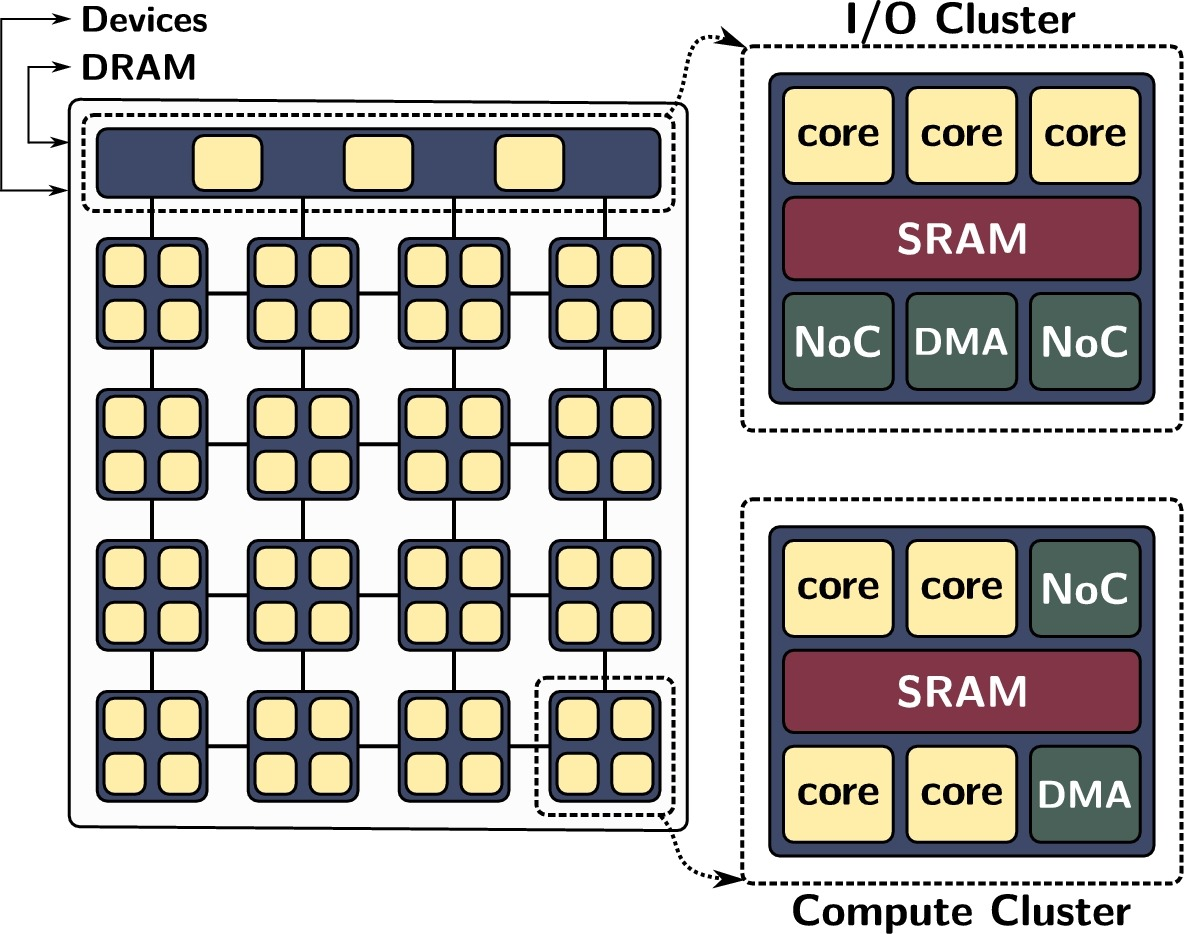
\includegraphics[width=0.64\linewidth]{content/images/lw-overview.jpg}
	\caption{Visão conceitual de um processador \lw \cite{penna2021inter}}
\end{figure}


Apesar de os processadores \lws serem uma alternativa às abordagens tradicionais no que se refere ao aumento de desempenho, as características arquiteturais ainda induzem problemas de programabilidade nas aplicações paralelas \cite{Castro-PARCO:2016}. Entre eles podem-se citar:

\begin{enumerate}[label= (\roman*)]
    \item Modelo de programação híbrida que força troca de informação entre os \clusters exclusivamente por troca de mensagens via \noc \cite{kelly2013};
    \item Sistema de memória restritivo, em que há multiplos espaços de endereçamento, pequena memória local, necessidade de busca em memória remote e separação da memória em pequenos blocos explicitament para a manipulação dos dados \cite{Castro-PARCO:2016};
    \item Latência e gargalos de comunicação na \noc;
    \item Falta de suporte de coerência de cache para economia de energia, o que exige do programador a gerência de cache via \software;
    \item Configuração heterogênea no que se refere aos \cclusters e \ioclusters, o que dificulta o desenvolvimento de aplicações;
\end{enumerate}

Atualmente, alguns estudos são feitos para amenizar o impacto da arquitetura sobre o desenvolvimento de aplicações. Neles, sobresaem-se os \oss distribuídos, que garantem um ambiente mais robusto e rico \cite{asmussen_m3:_2016, kluge_operating_2014, penna:sbesc19}. Destaca-se ainda os estudos em \oss ditribuídos baseados em uma abordagem \multikernel \cite{penna2017-1,penna2017-2,penna2019}.

Nesse cenário, a virtualização dos recursos do processador é importante para o suporte a multi-aplicação e para maior eficiência do mesmo \cite{vanz2022virtualizaccao}. Contudo, as características arquiteturais dos \lws, especialmente relacionadas à memória, inviabilizam um suporte complexo para virtualização. Por exemplo, máquinas virtuais utilizadas em ambientes \cloud possuem à disposição centenas de GBs para isolar duplicatas inteiras de \oss com a ajuda de virtualização no nível de instrução \cite{sharma2016containers}. Nos \lws, as pequenas memórias locais e a simplificação do \hardware para reduzir o consumo energético restringem os tipos de virtualização suportados.

Neste contexto, este trabalho trabalho explora um modelo mais leve de virtualização para \lw baseada em contêineres. Contêineres são executados pelo \os como aplicações virtuais e não incluem um \os convidado, resultando em um menor impacto no sistema de memória e requerendo menor complexidade do \hardware \cite{thalheim2018cntr, sharma2016containers}.

\glsresetall
\section{Objetivos}
\label{sec.goals}

Com base nas motivações citadas previamente. Os objetivos deste trabalho serão especificados nas próximas seções.

\subsection{Objetivo Principal}
\label{sec.goals.primary}

O objetivo principal deste trabalho é adaptar o \nanvix, um \os para \lws, de modo que os recursos utilizados por um processo sejam virtualizados. Isso com o objetivo de desvincular a execução de um processo com o local \ie \cluster onde está alocado e aumentar a mobilidade de processos no processador.

\subsection{Objetivos Específicos}
\label{sec.goals.secondary}

\begin{enumerate}[label= (\roman*)]
    \item Propor um modelo de virtualização adaptado às necessidades e imposições de um \lw;
    \item Implementar o modelo proposto no \nanvix, um \so distribuído para \lws;
    \item Analisar a corretude da solução através do desenvolvimento de \benchmarks que avaliem a migração de processos;
    \item Analisar o impacto do modelo de virtualização na execução normal do \nanvix;
\end{enumerate}

\section{Organização do Trabalho}
\label{sec.organization}

As próximas seções do trabalho estão organizadas da seguinte maneira. No \autoref{chap.background} serão apresentados alguns conceitos importantes para o melhor entendimento do trabalho. Dentre esses conceitos pode-se citar:
\begin{inlinelist}[label= (\roman*)]
    \item \Lws;
    \item Multiprocessadores;
    \item Multicomputadores;
    \item Virtualização.
\end{inlinelist}
Além disso, será detalhado o \os e o \lw que será utilizado neste trabalho.